%!TEX root = Main.tex
\section{Theory}
This section will contain a brief overview of the compression techniques used. It will also contain information on the TelosB mote platform.


\subsection{Image}
In this project a $256 \times 256$ pixel grayscale cameraman image (Figure \ref{fig:image_cameraman}) is used. 
The image is saved in the TelosB flash as a binary file. Each pixel is represented with one byte, which gives a grayscale resolution of 256 shades.

\begin{figure}[ht!]
\centering
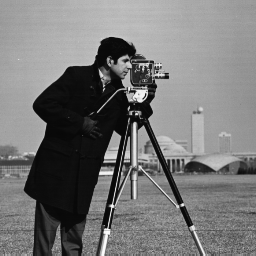
\includegraphics{cameraman}
\caption{Cameraman image used in the project.}
\label{fig:image_cameraman}
\end{figure}

\subsection{Energy Consumption}
Energy consumption is important when we look at wireless sensor networks. 
The component with the most energy consumption is the radio circuitry of the TelosB.
This can be seen in the TelosB datasheet\cite{dataSheet}. 
The challenge is to choose when to use the radio and how often. 
Comparing the radio current (23 mA) with the processing current (1.8 mA), it is indicated that a lot of processing is possible, before the power consumption gets larger than the cost of sending. 

\subsection{Compression}

Three different lossy compression algorithms is used in this project.
They have a simple implementation and are fast to compute, but they are not very good at retaining image quality compared to e.g. JPEG which uses discrete cosine transform and Huffman coding.

The algorithms are fast to compute since they mostly use cheap operations like bit swifting and bitwise AND/OR, and only iterates through the data once.
Lower computation time also means that the energy consumption is lower.

The compression algorithms work by throwing away the least significant bit/bits from every byte in the image.
For instance the four bit compression takes two bytes, \texttt{aaaa\_\_\_\_} and \texttt{bbbb\_\_\_\_}, and compresses them to a single byte \texttt{aaaabbbb}, where \texttt{a}, \texttt{b} and \texttt{\_} is a bit. Using this method, the image has been compressed 50\%.


\subsubsection{N-Bit Compression} % (fold)
\label{sub:one_bit_compression}

The N-Bit Compression gives a compression of $\dfrac{N\ bit}{8\ bit}$.
The algorithm takes 8 bytes and maps them into $8-N$ bytes where the N least significant bits, of each byte, is lost.

In this project N = \{1,2,4\}. The compression rate is seen in \ref{tab:compressionrate}.
\begin{table}[H]
	\centering
	\begin{tabular}{ll}
	\hline
		N & Compression rate \\ \hline
		1 & 12.5\% \\ 
		2 & 25\% \\ 
		4 & 50\% \\ \hline
	\end{tabular}
	\caption{Compression rates for N = \{1,2,4\}}
	\label{tab:compressionrate}
\end{table}
% \subsubsection{Two bit compression} % (fold)
% \label{sub:two_bit_compression}

% The Two Bit Compression gives a compression of $\dfrac{2\ bit}{8\ bit} = 25\%$.
% The algorithm takes 4 bytes and maps them into 3 bytes where the two least significant bits, of each byte, is lost.

% \subsubsection{Four bit compression} % (fold)
% \label{sub:four_bit_compression}

% The Four Bit Compression gives a compression of $\dfrac{4\ bit}{8\ bit} = 50\%$.
% The algorithm takes 2 bytes and maps them into 1 byte where the four least significant bits, of each byte, is lost.
